Con el fin de probar la mecánica y el desempeño de la inteligencia artificial se propuso un prototipo de 1.4m de ancho por 1m de alto útil. El mismo se planteó para ser trasladable por lo que se le dio una base y un respaldar para cumplir una función demejante a la de la pared.
\begin{figure}[H]
    \centering
        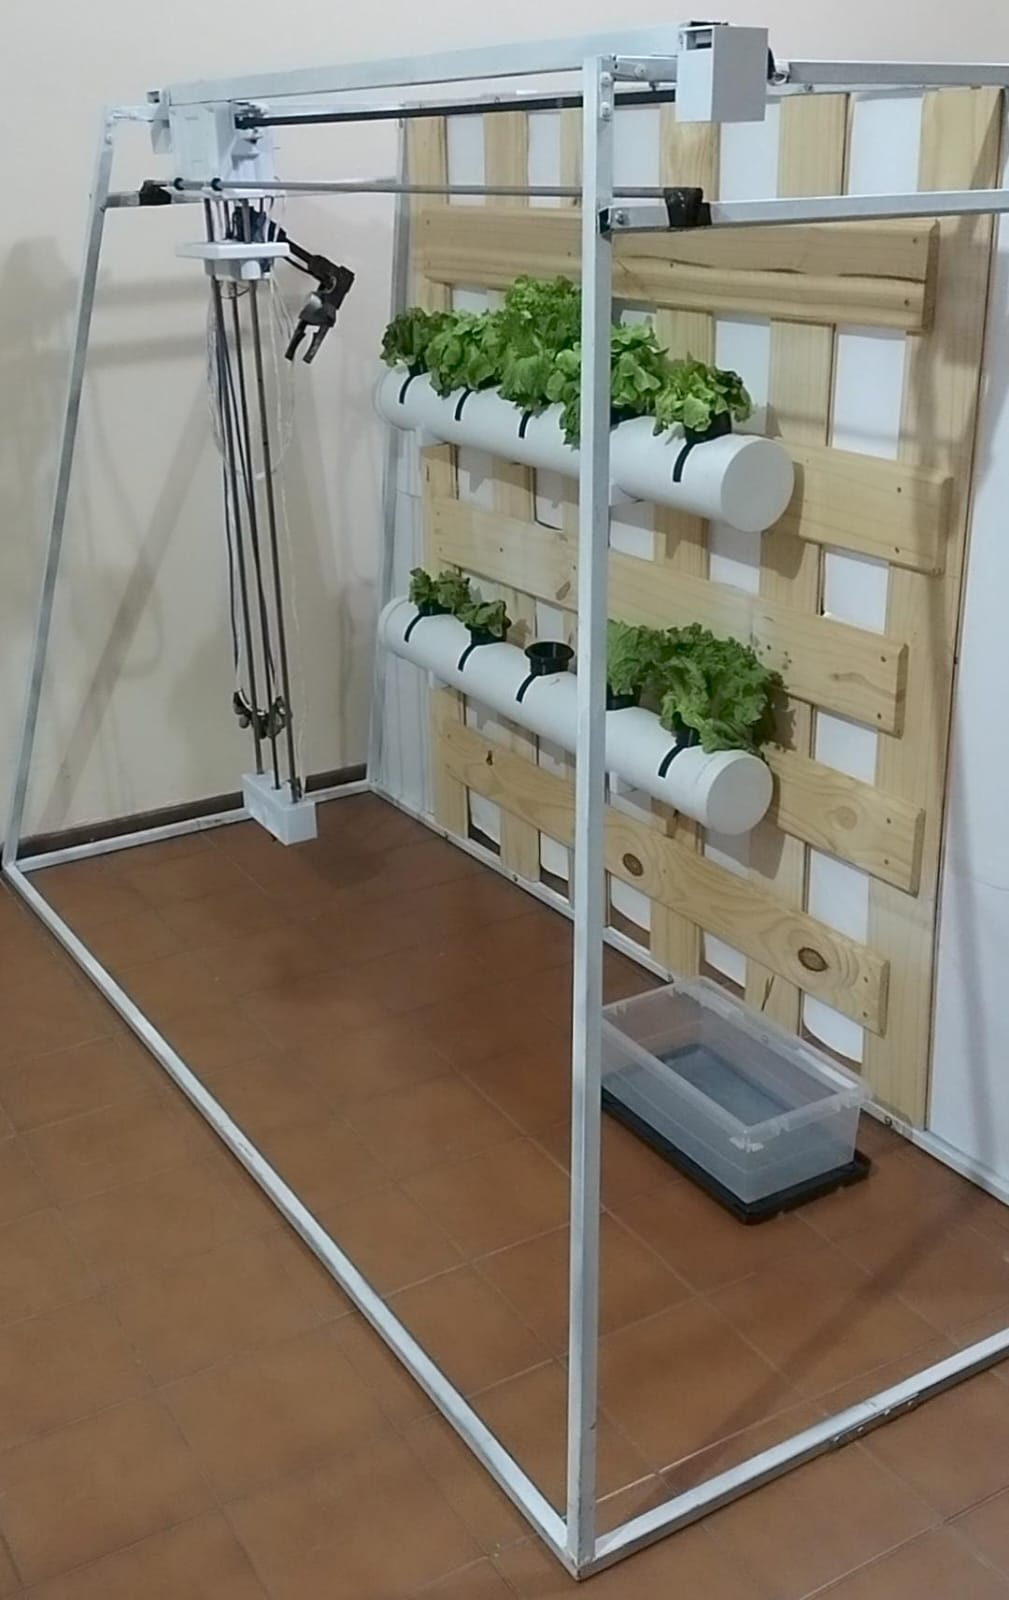
\includegraphics[width=0.65\textwidth]{img/estructura.jpg}
        \caption{\textit{Prototipo.}}
        \label{fig:estructura}
\end{figure}
La carga máxima horizontal es de aproximadamente 3.5kg mientras que la vertical es de aproximadamente 0.6kg.\\
Los parámetros cinemáticos son los de la tabla \ref{tab:especificaciones_cinematicas}.\\
En lugar del perfil v-slot y los carros que deslizan sobre él se opta por un perfil y dos carros semejantes al sistema de portones.\\
Como el sistema seleccionado es utilizado para cargas mucho mayores a la propuesta se presume que el perfil posee la rigidez necesaria para la aplicación.
\begin{figure}[H]
    \centering
    \begin{subfigure}{0.35\textwidth}
        \centering
        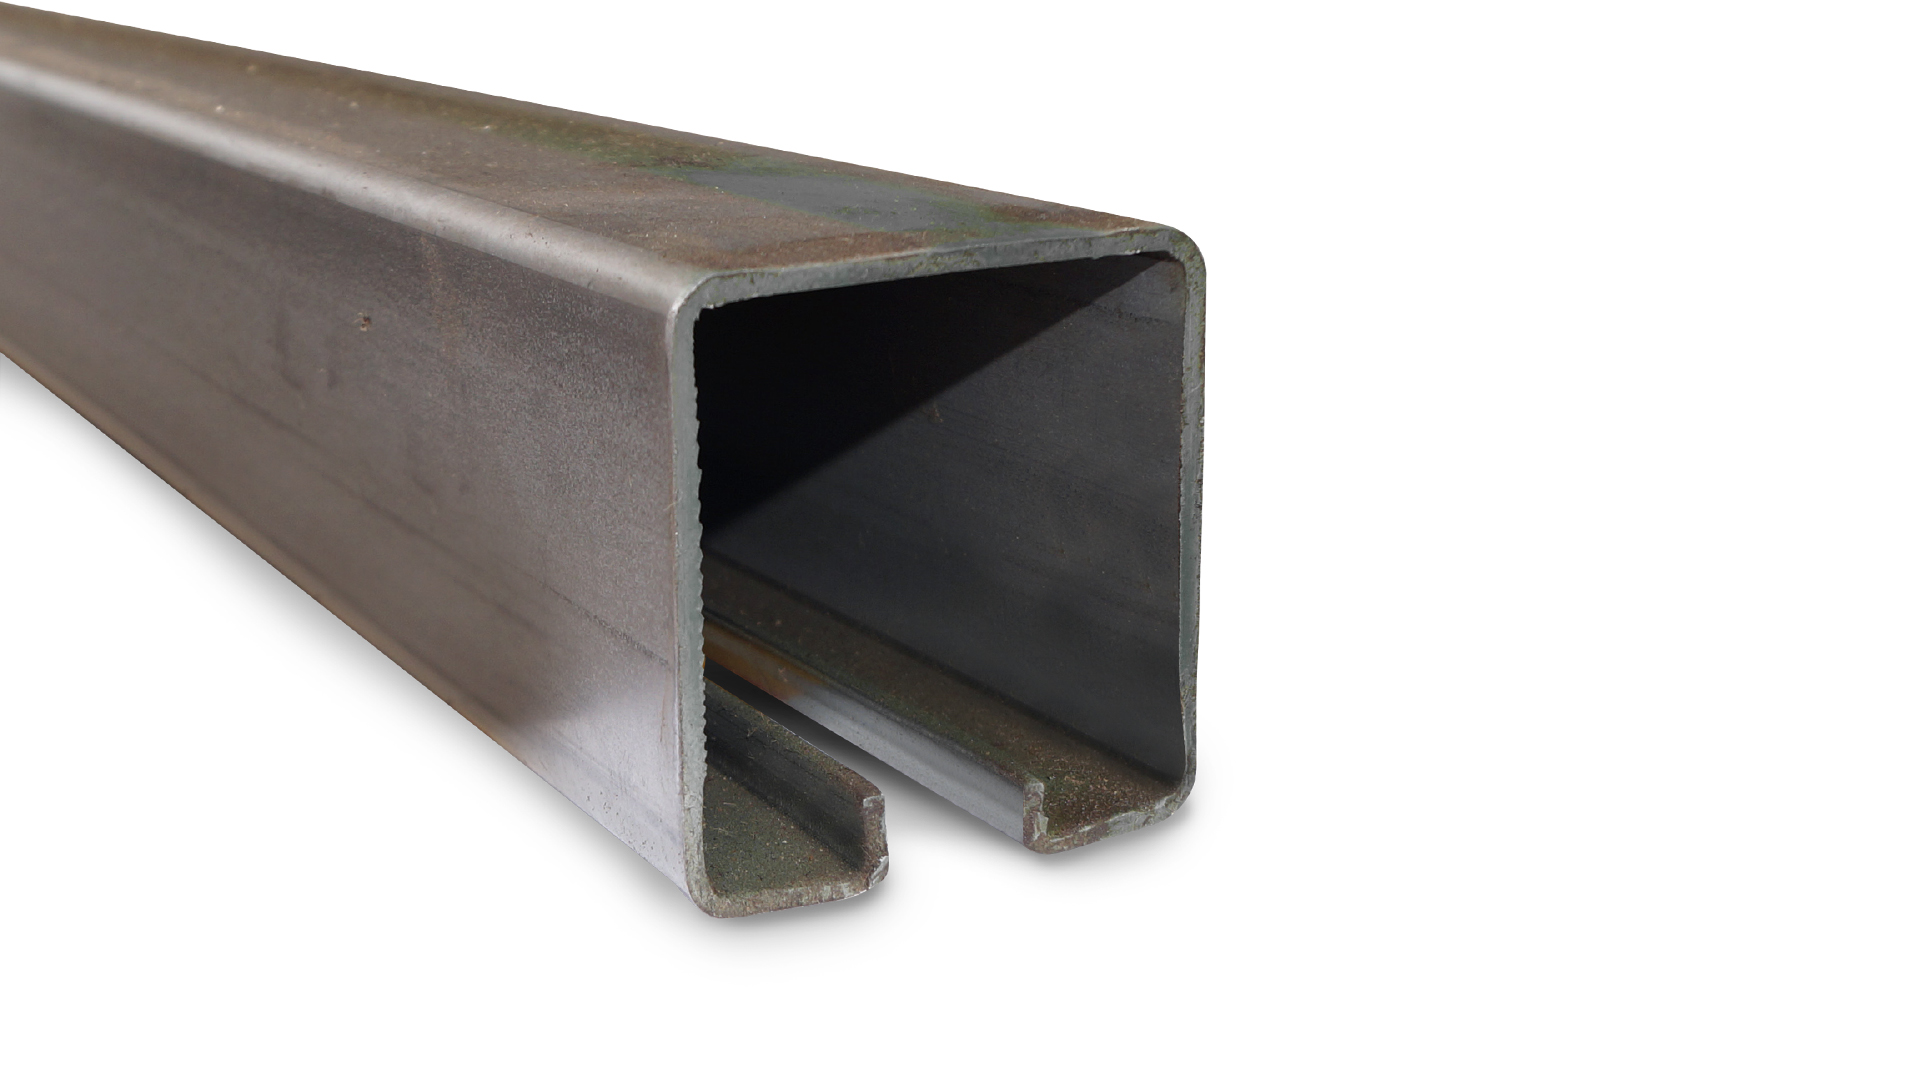
\includegraphics[width=\textwidth]{img/perfil_porton.png}
        \caption{\textit{Perfil utilizado en prototipo.}}
        \label{fig:perfil_porton}
    \end{subfigure}
    \hfill
    \begin{subfigure}{0.35\textwidth}
        \centering
        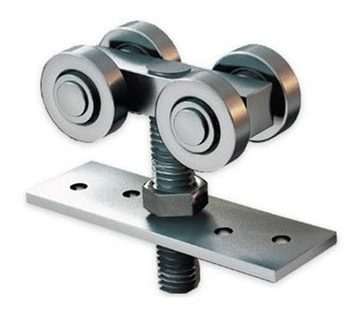
\includegraphics[width=\textwidth]{img/carro_porton.png}
        \caption{\textit{Carro para deslizamiento sobre perfil.}}
        \label{fig:carro_porton}
    \end{subfigure}
    \caption{Sistema de traslación horizontal.}
\end{figure}
Para el sistema de transmisión vertical se utilizo el mismo sistema que se describió en la sección \ref{sec:mov_vertical} pero de menores dimensiones, su correcta selección se justifica en los cálculos implementados en la sección \ref{sec:mov_vertical_prototipo}